% !TeX program = xelatex
% !TeX encoding = utf8
% !TeX root = RegT1E_HS22.tex

%% TODO: publish to CTAN
\documentclass[margin=normal]{tex/hsrzf}

%%%%%%%%%%%%%%%%%%%%%%%%%%%%%%%%%%%%%%%%%%%%%%%%%%%
% Packages

%% TODO: publish to CTAN
\usepackage{tex/hsrstud}

%% Language configuration
\usepackage{polyglossia}
\setdefaultlanguage[variant=swiss]{german}

%% License configuration
\usepackage[
    type={CC},
    modifier={by-nc-sa},
    version={4.0},
    lang={german},
]{doclicense}

%%%%%%%%%%%%%%%%%%%%%%%%%%%%%%%%%%%%%%%%%%%%%%%%%%%
% Metadata

\course{Elektrotechnik}
\module{RegT1E}
\semester{Herbstsemester 2022}

\authoremail{joel.leirer@ost.ch}
\author{\textsl{Joël Leirer} -- \texttt{\theauthoremail}}

% did someone help you with this work?
\contributors{
  % I created this template, does that count?
  Naoki Pross
  % do not forget to add yourself!
}

\title{\texttt{\themodule} Zusammenfassung}
\date{\thesemester}

%%%%%%%%%%%%%%%%%%%%%%%%%%%%%%%%%%%%%%%%%%%%%%%%%%%
% Document

\begin{document}

% use roman numberals for introductiory pages
\pagenumbering{roman}

\maketitle


% show the names of the people who contributed to this document.
% \section*{Contributors}
% \thecontributors

\section*{Lizenz}
\doclicenseThis

\clearpage
\tableofcontents

% actual content
\clearpage
\setcounter{page}{1}
\pagenumbering{arabic}

\section{Wichtige Funktionen}
\label{func}
\begin{tabular}{p{5cm} p{10cm}}
  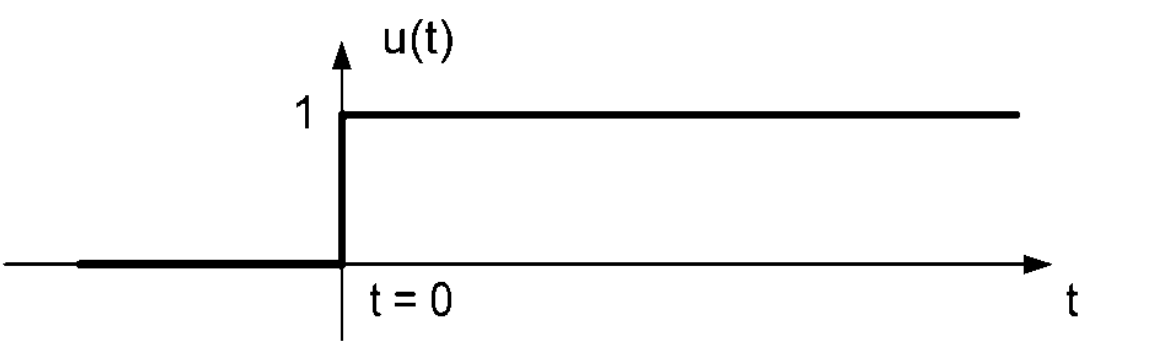
\includegraphics[width = 2.5cm]{img/Sprungfunktion.png} & 
  Sprungfunktion: \newline
  Normierter Einschaltvorgang \newline 
  $ t<0 : u(t) = 0, \ newline
  t \geqslant 0: u(t) = 1 $ \\

  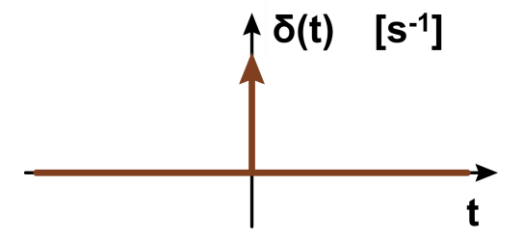
\includegraphics[width = 2.5cm]{img/Impulsfunktion.png} &
  Impulsfunktion = Deltafunktion = \newline 
  Diracimpuls = Delta-Distribution \newline
  Unendlicher kurzer normierter Impuls mit unendlicher Amplitude

  Mathematische Eigenschaften:
$\int\limits _{-\infty} ^{+\infty} f(t) \cdot \delta (t-t_0) dt = f(t_0)$ \newline
$\int\limits _{-\infty} ^{+\infty} f(t) \cdot \delta (t) dt = f(0)$\newline
$\int\limits _{-\infty} ^{+\infty} \delta (t) dt = 1$ \\
%TODO: Find Graphic 
&
$\varepsilon(t) = \begin{cases} 0$ für $ t<0 \\ 1 $für$ t \geq 0 \end{cases}$\\


\end{tabular}
\section{Begriffe}
\begin{itemize}
      \item Prozess
            \begin{itemize}
                  \item Die Gesamtheit zusammenwirkender Vorgänge, welche durch
                        die Materie, Energie und Information
                        umgefort, transportiert und gespeichert wird.
            \end{itemize}

      \item System
            \begin{itemize}
                  \item Ist gegenüber der Umwelt abgegrenzt, hat Eingänge,
                        Ausgänge (und Zustand).
                  \item (LTI-/)LZI-Systeme: Lineare-ZeitInvariante Systeme
                        (Linearität gilt, System ist unabhängig von zeitlicher Verschiebung
                        --> DGL mit Konst. Koeff.)
            \end{itemize}

      \item Modell
            \begin{itemize}
                  \item Beschreibung von Systemen, wird genutzt für
                        Erklärung, Prognose, Gestaltung und Optimierung.
                  \item Es gibt kein "richtiges Modell",
                        ein Modell beschreibt ein System nur so genau wie nötig.
            \end{itemize}
      \item Modellieren
            \begin{itemize}
                  \item Teilsysteme erstellen und diese
                        in weitere Teilsysteme aufzutrennen.
                        So erhält man einfache Grundsysteme (Grundglieder),
                        welche sich einfach Mathematisch beschreiben lassen.
                        Zusätzlich kehern einige Teilsysteme in ihrer
                        Struktur oft wieder und können wiederverwendet werden.

                  \item Top-Down: System in Teilsysteme teilen
                  \item Bottom-Up: System aus Grundglieder aufbauen
            \end{itemize}
      \item Grundglieder
            \begin{itemize}
                  \item Kleinste Teilsysteme. Sie können weiter augeteilt werden in, siehe Abschnitt \nameref{Grundglieder}
            \end{itemize}
      \item Sprungantwort
            \begin{itemize}
                  \item Reaktion des Systems auf die Sprungfunktion. Siehe \refname{func}
                        
            \end{itemize}
      \item Schrittantwort
      \item \begin{itemize}
                  \item Reaktion des Systems auf die Schrittfunktion. Siehe \refname{func}
            \end{itemize}
      \item Ausgleich
            \begin{itemize}
                  \item Prozesse ohne Ausgleich: Sprungantwort wächst Grenzenlos an
                  \item Prozess mit Ausgleich: Sprungantwort strebt endlichem Wert zu
            \end{itemize}

\end{itemize}

\subsection{Grundglieder}
\label{Grundglieder}
\begin{itemize}
      \item Statische Glieder(Systeme ohne Gedächtnis):
            Der Ausgang ist nur vom aktuellen Eingang abhängig.
            $y(t)=f(u(t))$
            \begin{itemize}
                  \item P-glied (Proportionalglied): Reagiert mit einem Faktor K auf den aktuellen Eingangswert.\\
                        $y = K \cdot u$
            \end{itemize}
      \item Dynamische Glieder (System mit Gedächtnis):
            Der Ausgang ist vom aktuellen sowie von vergangenen Eingängen Abhängig.
            Vergangene Eingänge werden im System als Zustand x(t) gespeichert.
            $y(t)=f(u(t),x(t))$ \\Können weiter unterteil werden in:
            \begin{itemize}
                  \item I-Glied (Integrierer):
                        Ausgangssignal ist Abhängig vom Integrierten Einganssignal, Allenfalls mit einem Faktor K multipliziert. \\
                        $y(t) = K \cdot \int \limits _{t=0} ^{t} u(\tau) d\tau + y(0)$ \\
                        $(\frac{dy(t)}{dt} =)$ \space $\dot{y}(t) = K \cdot u(t) $
                  \item Totzeitglied: Verzögert das Eingangssignal um die Totzeit $T_t$\\
                        $y(t) = u(t-T_t)$
                  \item PT$_1$-Glied:
                        LZI-Übertragungsglied mit Proportionalem Übertragunsverhalten \\
                        und Verzögerung 1. Ordnung. (Bsp. Tiefpass 1.Ordnung als RC-Glied)

                  \item PT$_2$-Glied
                        \begin{itemize}
                              \item %TODO:
                        \end{itemize}
                  \item D-Glied(idealer Differenzierer)
                        \begin{itemize}
                              \item %TODO:
                        \end{itemize}
                  \item DT$_1$-Glied
                        \begin{itemize}
                              \item %TODO:
                        \end{itemize}
                  \item PI-, PD- PID-Glied (PDT$_1$ und PIDT$_1$)
                        \begin{itemize}
                              \item %TODO:
                        \end{itemize}
                  \item Lead-Glied, Lag-Glied, Lead-Lag-Glied
                        \begin{itemize}
                              \item %TODO:
                        \end{itemize}

            \end{itemize}
\end{itemize}

\end{document}
